% vim:ft=tex
\section{Simulation approach}
\label{sec:simulation}
In this section, we describe how our simulation is implemented, and how the 
implementation works.

Our simulation is implemented in the Python programming language, with the 
calculation intensive parts implemented in C for performance reasons. We 
assume a virtual coordinate system using meters as a base unit, and with the 
origin in the centre of the area we simulate. Each pedestrian (or actor) is 
described by a centre point and a radius, and each wall is described by a line 
segment connecting two points.

All parameters are stored as double precision floating point values where 
nothing else is indicated. We use custom data structures to keep track of the 
actors and walls while running the simulation. Python is used to set up the 
initial conditions, run the program's main control loop, and draw the 
simulation results through the \emph{PyGame} library \cite{pygame}. This 
allows to do both real-time animation as well as saving each simulation step 
to be assembled into a film afterwards. All calculations and data processing 
is done in a Python extension written in C, to increase performance.

\subsection{Initial conditions and constants}
When initialising the model, parameters are set for each pedestrian. In the 
model, every parameter can vary between actors, while in practice many of them 
do not. In this section, we go through the parameters and how they are set.  
For all random numbers, the operating system's built-in random number 
generator is used and considered to be sufficient for our purposes. We run 
multiple simulations of the same initial conditions by fixing the seed of the 
random number generator to the same value for each run. Distributions are 
drawn by using the distribution functions of the \emph{NumPy} mathematical 
library for Python \cite{numpy}.

\subsubsection{Position related parameters}
There are a number of parameters that are set that has to do with the initial 
position of actors and walls. They are:

\begin{itemize}
    \item \textbf{Wall endpoints:} Points describing the endpoints of the 
        walls. These are set according to the scenario we want to simulate, so 
        in a square room with a single exit in the middle of a wall, there 
        will be five wall segments (one on each side of the exit, and one for 
        each of the other walls).

    \item \textbf{Actor positions:} Each actor has a starting position 
        distributed randomly within the room. These are created by drawing a 
        set of random numbers for the x and y coordinates respectively, and 
        adjusting the range of this random number to be within the room's 
        dimensions. Actor positions are adjusted so that they do not overlap 
        with the walls by adjusting coordinates so that the distance from the 
        center to each wall is at most the radius. This adjustment is not made 
        between actors, so they may overlap initially. It is assumed that the 
        model will correct this within the first few simulation steps, which 
        is also what we have seen in practice.

    \item \textbf{Actor radii:} The actor radii are drawn from a normal 
        distribution with a mean of $0,2$ meters and a standard deviation of 
        $0,01$ meters. This is done to simulate a natural variety in physical 
        stature of humans, and to avoid deadlocks caused by perfectly 
        symmetrical forces that might otherwise occur \cite{helbing00}.
        %TODO: Check this reference, maybe better explanation?
\end{itemize}

\subsubsection{Movement related parameters}
A number of parameters are set to control the movement of the actors. They 
are:

\begin{itemize}
    \item \textbf{Target:} Each actor has a target that they move towards. 
        This target is set outside the exit actors will move towards, and is 
        the same for all actors when there is only one exit. In situations 
        where there are multiple exits, actors are set to move towards one of 
        the exits at random, regardless of their position within the room. 
        Since the model does not deal with pathfinding, targets are not 
        changed during the simulation. When an actor reaches its target, it is 
        considered to have escaped, and is removed from the simulation.

    \item \textbf{Initial velocity:} This is set as both a vector and a scalar 
        representing vector length. The scalar velocities are drawn from a 
        normal distribution with a mean of $1.34$ and a standard deviation of 
        $0,26$. The initial velocity vectors are created by multiplying the 
        scalar velocity with a normalised vector pointing from the actor's 
        initial position to the target.
        % TODO: Where do the mean and deviation come from?

    \item \textbf{Max speed:} TODO.

    \item \textbf{Desired velocity:} The desired velocity is the velocity the 
        actor wants to move at (see the explanation in 
        section~\ref{sec:the-model}). This is set equal to the initial velocity 
        under the assumption that when people start to leave a room they will 
        initially (try to) move at their desired velocity, and then be 
        affected by the model parameters once they start moving.

    \item \textbf{Relaxation time:} The relaxation time is the time it would 
        take an unhindered actor to return to their desired velocity after 
        having been hindered by something blocking their path. This is set to 
        one second for all actors.
        % TODO: Why one second, and is this explanation correct?

    \item \textbf{$\lambda$:} \cite{self-org} chose $\lambda$ $\approx 0.75$ to take into account
	anisotropic character of pedestrian interaction, such that the situations in front of
	a pedestrian have bigger impact on the pedestrians behavior than things going on
	behind them. By looking at eguation 44 we see that if we set $\lambda = 1$, the middle 
	paranthesis will be 1, and hence the personal sphere will only take into account the distance
	between agent $\alpha$ and $\beta$ and not their placement respect to each other. By setting $\lambda = 0$, the middle paranthesis will be
	$\frac{1+\cos{\phi}}{2}$
	and therefore the situation happending behind agent $\alpha$ would affect $\alpha$'s behavior.
	By setting $\lambda \approx 0.75$, the first part of eguation 44 is
	 $A_{\alpha}^{1} exp \left(
            \frac{ r_{\alpha \beta} - d_{\alpha \beta }}
                 {B_{\alpha}^1}
	    \right)
	  \vec{\eta_{\alpha \beta}} \cdot
	  \left(
	      0.75 + 0.25
		\frac{1+\cos{\phi}}{2}
	    \right)$,
	and  other agents behind $\alpha$ will only influence $\alpha$ with 25\% of what the influence would be without a $\lambda$.
	Even though the model is called a social force model, we will point out that it is not physical forces acting on agent $\alpha$ but
	rather motivation to act. This is more clear when adding $\lambda$, since Newton's 3'rd law (action = reaction) does not hold
	when $\lambda$ priorities what forces and how much the forces should influence the agents.
\end{itemize}

\subsubsection{Constants}
The model includes a number of constants. These are parameters that do not 
vary between the agents, but are fixed for the whole simulation. They are:

\begin{itemize}
    \item \textbf{Timestep:} The timestep is the $\Delta T$ that passes for 
        each step of the simulation. As discussed in 
        section~ %TODO: Make new reference
		, there are various trade-offs in making 
        this parameter larger or smaller. We have experimented with different 
        values, and have found that a value of $0,01$ seconds make for a 
        simulation without errors such as jitter that results from larger 
        timestep values. Since setting the timestep corresponds to setting a 
        delta value for an Euler integration, there are various methods that 
        originate from this integration method, that might be used to vary the 
        timestep dynamically during the simulation. However, we have found 
        that with a fixed value of $0,01$ seconds, we get reasonable 
        performance of our simulation, so we have not found the need to 
        complicate our program by applying such methods.
        % TODO: Reference for dynamic timestep adjustment

    \item \textbf{$A_1$, $B_1$:} TODO.

    \item \textbf{$A_2$, $B_2$:} These values are given in \cite{helbing00}. 
        Although the model allows for them to vary between agents, we have 
        (just as is done in the article) set them to a fixed value for the 
        whole simulation. The values given are $A_2=3,0$ and $B_2 = 0,2$.
\end{itemize}

%The potential between pedestrian $\alpha$ and the wall $B$ is given by 

%\begin{equation}
%V_B=V_B^0 e^{-(r_\alpha - r_B^\alpha )/R} 
%\end{equation}
%where $V_B^0 = 10m^2s^{-2}$ and $R=0.2m$.
%These model parameters have been determined such that they are compatible with empirical data. 
%(Kilde: Dirk Helbing and Peter Molnar - Social force model for pedestrian dynamics). This is 
%the older article by Helbing, and it seems as if its the same initial conditions, as in 
%the article we are working with, except that the force between to pedestrians has changed. 
%But still I think we could use the old article to argue why these parameters 
%have the given values.\\

%\noindent
%$A^2_\alpha = 3m/s^2$ and $B^2_\alpha = 0.2 m\\$
%$A = 5 m/s^2$ and $B=0.1m$
%$r_{\alpha \beta} = 0.6m$
%$\lambda_a = 0.75$\\\\
%\noindent
%These values for the model have been calibrated with empirical data of pedestrian streams.
% TODO: What is this section doing here?

\subsection{The simulation steps}
The simulation is divided into two parts: Finding the accelerations (or 
resulting force) for all actors, and updating position and velocity for the 
actors.  Since the acceleration for each actor is dependent on both position 
and velocity of the other actors, splitting the calculations this way enables 
us to do the calculations of each actor in any order, and even parallel. The 
drawback is that the actors are only affected by the movement and positions of 
other actors as they were at the end of the last simulation step. This means 
that the time step has to be small enough that this doesn't matter in 
practice.

\subsubsection{Calculating the acceleration vectors}
The acceleration vectors for each actor, $\alpha$, is calculated as follows:

\begin{enumerate}
    \item Determine the acceleration vector provided by the actors' desired 
        direction of movement.
    \item For each other actor $\beta_1\dots\beta_n$, calculate the 
        acceleration vector provided by avoiding the actor $\beta_i$.
    \item Calculate acceleration vectors resulting from avoidance of the walls 
        $w_1\dots w_n$.
    \item Sum all the acceleration vectors to a resultant acceleration vector 
        $a$.
\end{enumerate}

Steps one to three correspond to the three parts of the model.

\subsubsection{Calculating the repulsion from walls}
The calculation of repulsion from the walls is split in two parts for each 
actor: First all the points on the walls that will affect the actor is 
identified, then the repulsion from each point is calculated. As explained in 
section~\ref{sec:the-model}, the repulsion from the wall is measured from the 
nearest point of the wall to the actor. Identifying these points is done using 
the following algorithm:

\begin{enumerate}
    \item For each wall, calculate the projection of the vector pointing from 
        the wall's starting point to the actor, unto the vector pointing from 
        the wall's starting point to its endpoint.
        \begin{enumerate}
            \item If this point is part of the wall, save it to the list of points 
                repulsion should be calculated from, and add the wall's two endpoints 
                to the list of already used endpoints.

            \item If the projected point is not part of the wall, the endpoint closest 
                to the actor is used instead. This endpoint is saved to a 
                third list of endpoints repulsion should be calculated from.
        \end{enumerate}

    \item After having gone through all walls, for each point in the third 
        list, check if this point is already in the list of used endpoints. If 
        so, discard it. Otherwise, add it to the list of points repulsion 
        should be calculated from, and to the list of used endpoints.
\end{enumerate}

The algorithm starts out with the list of walls, and produces a list of points 
to calculate this repulsion from, ensuring that no wall endpoint is used 
twice. The points are then used as a basis for calculating the repulsion, as 
described in section~\ref{sec:the-model}.

\subsection{Updating position and velocity}
After every actor has been updated with a resulting acceleration vector from 
the current simulation step, all actors update their position and velocity.  
The position is updated by calculating a displacement vector as follows:

\begin{equation}
    \Delta p = (v_x \Delta t + \frac{1}{2}a_x \Delta t^2, v_y \Delta t + 
    \frac{1}{2}a_y \Delta t^2)
\end{equation}

Where $v_x$ and $v_y$ are the $x$ and $y$ components of the velocity vector, 
$a_x$ and $a_y$ are the $x$ and $y$ components of the acceleration vector, and 
$\Delta t$ is the time step.

After updating the position, the actor's velocity is updated by adding the 
acceleration vector, to be used for the next simulation step.

% start parameters: p_n, v_n for each person.
% p for each wall
%
% steps:
%
% for each person:
%   calculate acceleration from the force parts of the model
%
% for each person:
%   update position by displacement vector
%       delta-p = (v_x*delta-t+1/2*a_x*delta-t^2, 
%       v_y*delta-t+1/2*a_y*delta-t^2)
%   update velocity for next step
%
%
% initial parameters:
%   Set using some sort of distribution around a mean
%
%
% constants:
%   Where do they come from?

\subsection{Measurement of the concepts flow rate, density and efficiency}
As mentioned in section \ref{concepts}, we want to have some concepts we can use to compare
the simulations and to see if the simulations make sence.
In this section we will describe how we want to measure the concepts efficiency,
flow rate and density.

\textbf{Efficiency}
We will measure the efficiency throughout the simulations. The efficiency is a 
dimensionless number given by the average speed of each pedestrians divided by 
the desired speed of each pedestrian. We will meassure the avereage speed in each 
timestep as:

\begin{equation}
	\overline{V_t}=\frac{1}{N}\sum_{i=1}^{N}V_i
\end{equation}
Where $V_i$ is the speed of the i'th pedestrian and N is the number of pedestrians 
still left in the simulation(Since there is no reason to include pedestrians who have 
reach there desired point since they are not moving). Then to find the efficiency for 
the entire simulation we make a summation of $V_t$ for each time step and then divide 
with the number of simulation steps. So given as an equation we have

\begin{equation}
		E=\frac{1}{T}\sum_{t=0}^{T}\frac{\overline{V_i}}{V^0_{i}}
\end{equation}

Where T is the number os simulations step and $V^0_{i}$ is the desired speed. This will 
give us an meassure about how fast the avereage speed the pedestrians where moving. In 
crowed simulations one should expect the efficiency to go to zero since people won't move 
fast and in a low density simulations it should be expected to have a value close to one $1$. 
The efficiency will in some way be a more general measurement of how fast pedestrians move 
throug a simulation than say the time it takes for the pedestrias to leave a room. Because 
the time will be strongly depenten on the shape of the area in the simulation and will be 
hard to compare with another situation. 
	
\textbf{Flow rate}
Part of the model geometry was made as a line seqment where we measure the average flow 
rate and the maximum flow rate, as pedestrians crossing the line seqment per second. 
This line should of course be placed somewhere the pedestrians actually are moving through. 
So in the case of a squared room you could place the line in the doorway that people move 
through when leaving the room. Also you could place more than one line and see if there is 
a difference in the flow rate throughout the room.   When we meassure it we will againg have 
to be carefull with the time onwhich we meassureit. The time step length that we have chosen 
to use in the simulations is $0.01$s. This is very small when meassuring the flow rate because 
the pedestrians will be more than $0.1$s about crossing a line completly(I.e. a pedestrian 
with a radius of $0.4m$ will move at a speed of $40$m$/$s if he where to cross the line in 
one time step). So in many step the flow rate would then be zero and then suddenly $100 s^{-1}$ 
when just one pedestrian has crossed the line. On the other hand it would be just as bad to 
meassure it every time 20 second has gone since all the pedestrian might have crossed the 
line and maybe they did it in only 10 seconds. So it is important to choose the right time 
when meassuring the flowrate. We have chosen to measure it for each second, that is every 
time we have done $100$ time steps. This requires a pedestrian to move at $0.4m/s$ to 
entirely cross the line. Also we will calculate the flow speed for the entire simulation. 
This we will measure as the number of pedestrians who have crossed the line in the time 
that it took for the last pedestrians to cross the line.      
	
\textbf{Density}
Another thing that we want to measure is the density of the pedestrians. When we do this, 
it of course makes no sence to measure the density of the entire area we make the simulation 
on, because then it will only change when a pedestrian leaves the simulated area. What we will 
do to makes is usefull is that we will choose a certain area on wich we will measure the density. 
In the case of a squared room it would be intersting to measure on an area of a couple of square 
meters just before the door that the pedestrians are leaving through. A sketch of this can be seen 
on figure \ref{fig:density}   
	
\begin{figure}
\centering
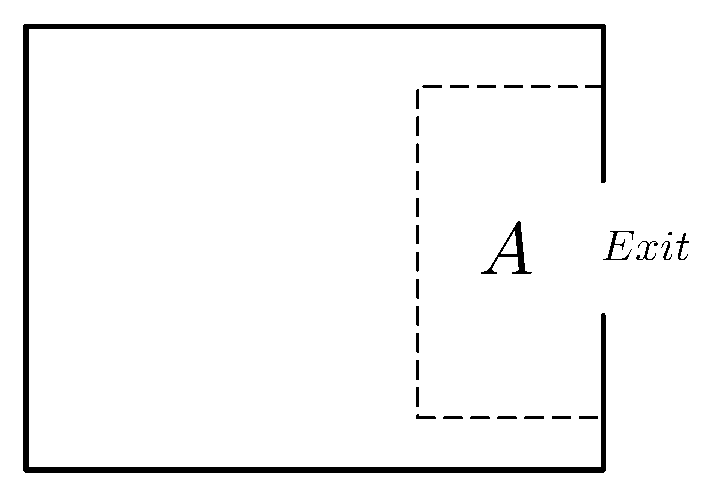
\includegraphics[scale=.5]{Figures/SquareCase.pdf}
\caption{Here is a sketch of the area that we want to measure the density on when simulating a squared room.}
\label{fig:density}
\end{figure}

So when we do the measurement it will be given as the area covered by the pedestrian 
divided by entire area on wich we measure the density. So the density will, as the 
efficiency, be a nondimensional number. Is will give us a more precise density than 
if we measured the number of pedestrian in the same area.  Becuase the pedestrians 
who are standing on the edge of the area but not completly inside, will notaffect 
the density. The measure of the density we will use to compare with the flow rate 
an see if the two are correlating when doing a simulation. It would be expected 
that when the flow rate goes down the diensity goes up in value. But it could be 
interesting to see it it i the same an se if there is some linearity between the 
two. This of coures implies that the area we choos will also be where we put the 
line that the pedestrians will cross when measuring the flow rate.   